\chapter{Discussion}\label{chap:discussion}
This chapter will discuss the obtained results, the used methodology, the validity and the reliability of the experiments, adapting the structure proposed by \textcite{luckert2016using}. Section \ref{sec:results-interpretation} will look into the results, describing what has been achieved, as well as indicate the main problems concerning the experiments. Section \ref{sec:method-reflection} will reflect on the research task and discuss whether the right method was chosen to solve the given task. Finally, Section \ref{sec:results-reliability} discusses the validity of the datasets that were used and the overall experiment setup. Based on these validity remarks, this chapter will clarify the reliability of the experiments' results. Therefore, the following questions will be tackled:
\begin{itemize}
    \item What conclusions can be taken from the presented results?
    \item Was the chosen method appropriate for the task?
    \item What benefits and shortcomings have been identified related to the presented work?
    \item What is the validity and reliability of the used data sets and the presented results?
\end{itemize}

\section{Results Interpretation}\label{sec:results-interpretation}
The best results among all algorithms were achieved by the manual manipulation of features "MAV", with a 0.67 cm error with a standard deviation of 2.46. The variations of MAV do not show substantial differences, yet they all present an average error higher than 0.5 mm with respect to the ground truth. 

This contrasts with the performance shown by the other two algorithms: RANSAC and DOPE. First, RANSAC could not match the pixel descriptors for the cow teats in the RGB images as shown in Section \ref{sec:results-research-question}. It is suspected that RANSAC could show better results if some preprocessing is done on the depth images. In other words, if the hypothesis that RANSAC cannot match figures of uniform colors from the RGB image, then a better performance could be seen when processing the depth image or the point cloud, as other research proposes \cite{papazov2010efficient}. Second, DOPE's performance was unexpected since it was used before for 3D recognition of chairs at the ZHAW and it showed promising results. It is suspected that DOPE's disappointing performance is originated because of the lack of photorealism in the materials of the data sets. Since the artificial cow teats materials are not a plain "gray", it was difficult to close the reality gap with simple materials. The hypothesis for improvement is that DOPE should show a better performance if the reality gap in the data set is minimized further.


An additional point of improvement would be a mechanism to reduce the offset error shown by "MAV". The correlogram shown in Appendix \ref{appendix:correlogram} was generated with the outputs from the algorithm, to obtain the correlation coefficients between the errors in (x, y, z) with the camera position (x, y, z) and the camera's direction (quaternion). The coefficients proved there is a strong indirect correlation between the errors and the camera metrics. Consequently, a linear model was fit to predict the errors based on the interaction of camera information variables. The model's adjusted R-squared shows that 94\% of the variation in the output variables is explained by the input variables. Additionally, the overall F-statistic of the model show that the model indeed provides a better fit than the intercept-only model. Finally, as shown in Figure \ref{fig:r_error_asf_xyzquat}, the model's residuals were analyzed. These show a constant error, constant variance, normal distribution and no influential outliers. All these cues hint towards the possibility of using a linear model to predict the error in the "MAV" algorithm to reduce the offset error in the final pose estimations.

 \begin{figure}[h]
        \centering
        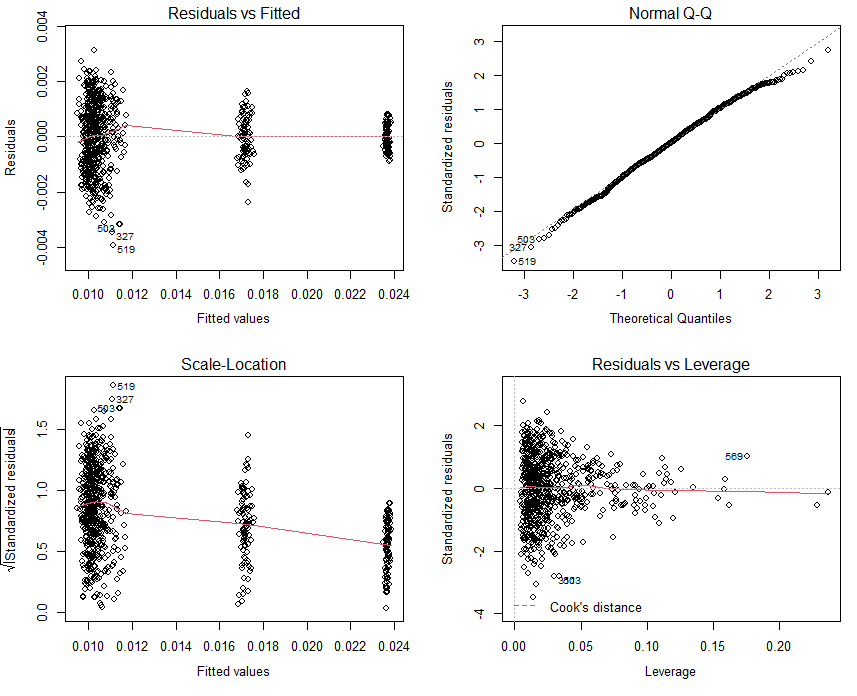
\includegraphics[width=0.8\textwidth]{images/r_error_asf_xyzquat.png}
        \caption{Linear model residuals of the model fit to predict the error from "MAV".}
        \label{fig:r_error_asf_xyzquat}
\end{figure}
    


\section{Method Reflection}\label{sec:method-reflection}
The used method, adapted from the work by \cite{luckert2016using}, proved to be appropriate for proposing a solution for the research question given. The structure provided allowed for the setup of different experiments without neglecting the initial goal. From the identification of the goal, through the data description and the specification and proposition of the computer vision approaches, the method proved to efficiently structure the work required to construct a pose estimation algorithm using machine learning.

\section{Reliability}\label{sec:results-reliability}
This section aims to discuss the validity and reliability of the results shown in section \ref{sec:results-research-question}.

The achieved results by the pose estimation algorithm, specially the adaptations done in contribution based off this work, show better performance than the methods in the market for the cow milking robots. The obtained results show promising a performance for current challenges like detecting two cow teats as one. Once the error in the proposed method is reduced, the proposed pipeline could be connected to a memory system that would keep track of the cow teat positions in cases of obstruction from the suction cups, as discussed in Section \ref{sec:future-work}.

In contrast, a few shortcomings related to the achieved results must be mentioned. First, the RANSAC algorithm analysis was limited to RGB images and should have been expanded to evaluate the information from the depth image and the point cloud. Second, a more photorealistic data set should be generated to show DOPE's prediction capabilities and carry out a proper comparison with the "MAV" algorithm. Third, the search space of the parameters adjusted should be wider and not limited to the ones presented. In conclusion, the "MAV" algorithm answers the research question with success, being able estimate the 3D pose and direction of a cow teat in less than 2 seconds.

\chapter{Conclusion}\label{chap:conclusion}
\section{Conclusions}\label{sec:conclusions}
This work answered the following research question:
\begin{itemize}
    \item How can the cow teats 3D pose be estimated under 10 seconds?
\end{itemize}
This was done by constructing a data set, training a segmentation algorithm and estimating the pose of the cow teats from the image and the predicted segementation masks. The images for the data set were collected from an artificial cow at the ZHAW using ROSBags to manually export frames at specific timestamps. The images were subsequently annotated and added to the data set. The model was then trained and tested using the generated data set. The false negatives and false positives indicated that more pictures at specific time stamps and positions with respect to the artificial cow had to be added to the data set, to increase the model's accuracy. Consequently, a pipeline was constructed for the independent deployment of the segmentation network and the pose estimation algorithms. The segmentation network would predict and publish segmentation masks for the pose estimation component to consume them and predict, in conjunction with the input images, the pose estimation of the observed cow teats. The methods tested were RANSAC and a manual manipulation approach "MAV". The latter contributed to two other approaches at the ZHAW for the pose estimation of cow teats. From the methods presented in this work, the best results were by a manual approach "MAV", which had a 0.67 cm error with a standard deviation of 2.46. 

Additionally, an Unreal Engine 4 project for data set generation was constructed for further research. It contains 5 photorealistic scenes with present parameters for rotations and obstructing objects. Finally, a synthetic data set of cow teats was generated with over 400k images for pose estimation. This dataset was used to train the pose estimation algoritmh DOPE, which unfortunately could not close the reality gap and output predictions from real images.

\section{Where to Go From Here?}\label{sec:future-work}
This work presents a pose estimation system for cow teats using machine learning and computer vision methods. There are a few possible routes for the extension of this work to improve the performance of the achieved results. First, a different segmentation network with a faster prediction time could significantly reduce the overall performance time of the presented approach, leading to almost real-time performance. Second, a memory system could help in cases of obstruction. For example, when the suction cups are attached, the system could still remember the position of the cow teats and attempt to reattach in case one of the cups detached on movement. Third, an active vision system could significantly improve the algorithm's time to obtain precise predictions. An active vision system would control the camera position and movement to collect frames with the least amount of movements, so that the objects in the scene could be remembered and understood more efficiently.

In conclusion, the presented work extends the related research on this topic by a providing machine learning and computer vision based approach for the 3D pose and direction estimation of cow teats.

% In this work we could show that is it possible to acquire a deep scene understanding from sequential
% data with supervised learning. In a simplified use-case such as the presented one, the system can
% successfully acquire a spatial scene understanding that includes objects, their shape, color and even
% their relationship with other objects. Although it is limited to the type of scenes the system was trained
% on, its versatility exceeds by far current mainstream object recognition systems such as ResNet [6].
% Unlike encoder-decoder-based scene understanding approaches such as [32], we do not need specified
% 3D models for training but only a simple scene description that specifies present objects including their
% positions and the camera poses of the captured images. 

% We could show that our system is capable of
% sequentially integrating information from new frames into the existing scene embedding vector. This
% capability is indeed highly remarkable because it includes the achievement of multiple non-trivial steps:
% 1.The change in camera position relative to the previous frame needs to be evaluated. The system does
% not receive any information about the camera position or rotation in space, but needs to extract this
% information based on the difference between the already perceived and the new input frame.2.This
% extracted transformation of the camera position must be used to transform all remembered object
% positions. Some objects might be occluded by the obstacle or other present objects, and the system is
% not able to perceive these items in the current frame. Nonetheless, it is necessary to transform their
% remembered positions so that the system is able to return the correct position when queried. The
% precision of this process however, would need to be further improved when used for robotic grasping,
% as there is still an average deviation of 0.11 meters (about half the diameter of the object) from the
% ground truth when using the best performing approach.

% While our proposed system does not use separated streams for ventral and dorsal pathways, our information
% aggregation process is inspired by the quicker decaying dorsal memory and the more persistent
% ventral memory. This is represented by learned weights versus aggregated temporary information. This
% architecture seems to work great, especially with respect to the 3 different shortcomings that were the
% focus of this work (see section 1.2). In the following, we discuss how our system overcomes them:
%     % \begin{itemize}
%     %     \item 1 paragraph big: describe what was achieved
%     %     \item 1 paragraph: describe our limitations
%     %     \item describe how we "overcame" the shortcommings: 3 paragraphs
%     %     \item closing remarks
%     % \end{itemize}


% \section{Towards Active Vision}
% Since this work was initially inspired by robotic interaction, we would see it as the next step to combine
% our vision-focused system with grasping approaches. An interesting direction would be to work towards
% solving benchmarks for robotic interaction such as RLBench [59].

% When approaching such tasks, we mainly see two possible paths to take: One relatively simple way
% would be to keep the perception and the grasping system separate and only use the output of the
% presented approach as input for a grasp generation algorithm, such as Dex-Net [60]. This would mean
% that the perception part would identify the target object and then forward its position to the grasp
% planning mechanism which would plan the grasp and pass it to the robotic arm for execution. As
% second option it would be possible that the condensed scene representation produced by our system
% would be beneficial for grasp-generation. We think that a promising approach would be to train two
% streams for grasping. The first stream could create a large number of possible grasps, while the other
% one would rate them with likelihood of success. Of course, the system would first need to learn to
% include the required information in the scene representation, which might be a large leap compared to
% the information currently present within the trained system. However, with the human mind closely
% coupling perception and action as part of the dorsal pathway it seems that such a joint approach could
% work for robotic grasping too.
%     % \begin{itemize}
%     %     \item 1 big paragraph describing how active vision could improve accuracy and object permanence
%     % \end{itemize}
% \section{Where to Go From Here?}
% While the discussed approach successfully solves the tasks set, the system is still far from being a real
% replacement for existing computer vision algorithms in use. On the way to the application of a system
% like ours to solve tasks in the real world, it would be necessary to solve at least some of the following
% challenges:

% Real world data: In order to use an approach like the one presented in a real-world use-case, it would
% above all be necessary to transfer the approach to real data or at least more realistic synthetic data.
% With the goal to jointly improve both scene understanding and active vision, we would inspire future
% research to use real-time data gathering with simulated environments as for example Isaac Sim [61].
% This would allow non-discrete view-positions and thus a potentially better understanding. One aspect
% that still might not be solvable by using synthetic data is the noise of the depth-channel of the RGB-D
% data, which is quite prominent for most consumer class RGB-D-camera.

% More different object classes/shapes: The presented solution uses only 5 primitive shapes with 7
% colors, which most likely does not reflect the conditions of a real world use case. A possible solution
% could be the use of large-scale 3D object data sets as used for Dex-Net [60]. Closely related to more
% diverse objects would be the capability to deal with duplicate objects. This could possibly be solved by
% adding multi-object output to all streams (as demonstrated with the Enumerating stream).

% Motion: In this work, we did not address the topic of motion, which does play a big roll in the real
% world. Environments like conveyor belts would be a domain where a scene understanding system like
% the one presented could prove highly useful. However, an application in such an environment would
% require previous research with dynamic scenes.

% Rotation axis detection: With only primitive objects such as cube, cylinders, etc., we decided not to
% include rotation information for our streams. However, for a large number of use cases it could be very
% useful to obtain the rotation of an object, so we would encourage future work to extend our approach
% to include rotation information.
% Grasping/bounding-box detection: For an actual application of robotic grasping, it would be necessary
% to generate possible grasping positions. We did not address this topic in the course of this work
% but leave the extension of the presented approach with grasping to further research. For more details
% see section 5.3.
%     % \begin{itemize}
%     %     \item describe in 5 small paragraphs 5 different future improvements for the voerall system
%     % \end{itemize}


